\pagebreak
\section{Project Dependent Preparations}

This section will describe, in \textbf{1-2 pages}, your preparations, progress and preliminary results (assuming you have relatively few at this stage). This section should include:

\begin{itemize}
    \item Evidence of training on specific equipment and/or upskilling in new software/methods
    \item Preliminary results/sketches
    \item Components/parts ordered
    \item Detailed budget of parts to be ordered
    \item Risk Assessment
\end{itemize}
In terms of preliminary results, you are encouraged to present your findings with graphical aids (figures, see example below).

%Figures can be created as shown below
\begin{figure}[H] % [H] positions the figure "here". For more information of positioning of Figure see: https://www.overleaf.com/learn/latex/Positioning_of_Figures and inserting an image here: https://www.overleaf.com/learn/latex/Inserting_Images
    \centering %Centres the figure in the middle of the page
    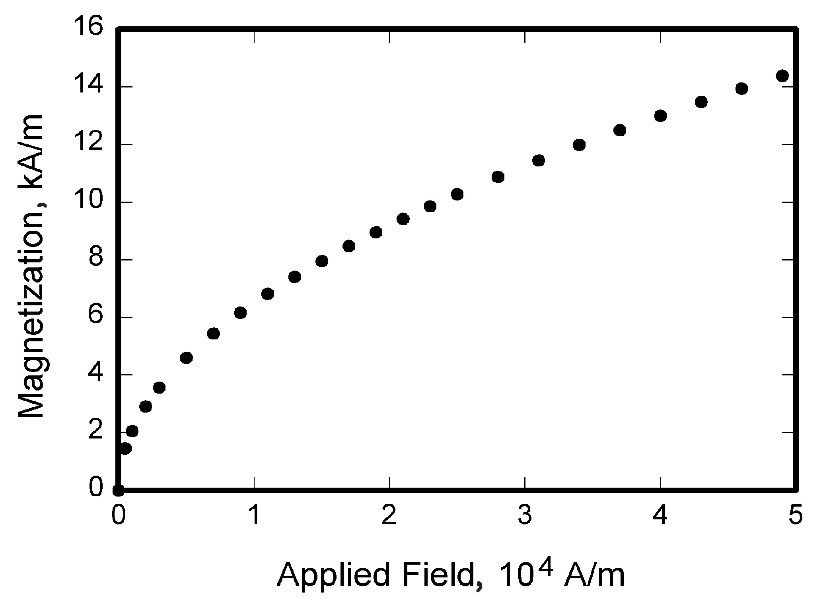
\includegraphics[width=10cm]{Figures/Image 1.jpg} % inserts the figure from the Figures folder (note figures need to be uploaded before inserting).
    \textbf{\caption{Magnetization as a function of applied field. \normalfont{\textit{Figure captions should be bold and justified, with a period and a single tab (no hyphen or other character) between the figure number and the figure description. If you took a figure from another paper or the web (when permitted), you MUST include a reference in the caption)}}}} %Captions can be included using \caption
\end{figure}

\begin{figure}[H]
    \begin{center} % Another option to centre the figure
        \subcaption[Dog] % If multiple images are required in a figure, the sub caption option can be used 
        {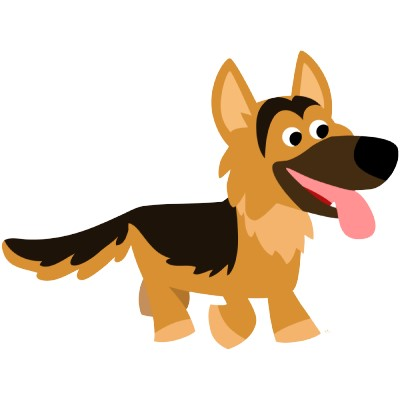
\includegraphics[width=0.24\textwidth]{Figures/Dog.jpg}} % The first image is include with size defined
        \subcaption[Doge] % Name of the subcaption is defined here
        {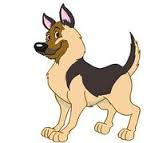
\includegraphics[width=0.24\textwidth]{Figures/Dog 2.jpg}} % The second image is include with size defined
        \textbf{\caption{Some Dogs}} % The overall figure caption is defined here
    \end{center}
\end{figure} 

% Tables can be created as shown. Tables can be generated with Latex syntax here: https://www.tablesgenerator.com/ 
% More information on creating tables can be found here:https://www.overleaf.com/learn/latex/tables
\begin{table}[H]
    \textbf{\caption{A Table}} %Table captions are placed above the table
    \begin{center} % Centres the table
    \begin{tabular}{ |c|c|c| } 
    \hline
    1 & 2 & 3 \\ 
    4 & 5 & 6 \\ 
     7 & 8 & 9 \\ 
    \hline
    \end{tabular}
    \end{center} 
\end{table}

Tables and figures of all types can be added inline or with text wrapping frames. Place figure captions below all figures; place table titles above the tables. If your figure has multiple parts, include the labels “a),” “b),” etc. below and to the left of each part, above the figure caption. Please verify that the figures and tables you mention in the text actually exist. 

When citing a figure in the text, use the abbreviation “Fig.” except at the beginning of a sentence. Do not abbreviate “Table.” Number each different type of illustration (i.e., figures, tables, images) sequentially with relation to other illustrations of the same type.

Figure axis labels are often a source of confusion. Use words rather than symbols. As in the example in Fig. 1, write the quantity “Magnetization” rather than just “M.” Do not enclose units in parenthesis, but rather separate them from the preceding text by commas. Do not label axes only with units. As in Fig. 1, for example, write “Magnetization, A/m” or “Magnetization, $Am^{-1}$,” not just “A/m.” Do not label axes with a ratio of quantities and units. For example, write “Temperature, K,” not “Temperature/K.”

Equations are centered and numbered consecutively, with equation numbers in parentheses flush right, as in Eq. (1). 

% Equations are defined as shown below
\begin{equation}
    \label{simple_equation} % Labels can be used to cross reference. For more information see: https://www.overleaf.com/learn/latex/Cross%20referencing%20sections,%20equations%20and%20floats
    Re = \frac{\rho\,UL}{\beta} % Equation is written here
\end{equation}

Be sure that the symbols in your equation are defined before the equation appears, or immediately following. Italicize symbols (T might refer to temperature, but T is the unit tesla). Refer to “Eq. (1),” not “(1)” or “equation (1)” except at the beginning of a sentence: “Equation (1) is…” Equations can be labeled other than “Eq.” should they represent inequalities, matrices, or boundary conditions. If what is represented is really more than one equation, the abbreviation “Eqs.” can be used.

Define abbreviations and acronyms the first time they are used in the text, even after they have already been defined in the abstract. Very common abbreviations such as CFD, SI, ac, and dc do not have to be defined. Abbreviations that incorporate periods should not have spaces: write “P.R.,” not “P. R.” 